\title{Kvik bestun}
\author{Bergur Snorrason}
\date{\today}

\begin{document}

\frame{\titlepage}

\env{frame}
{
	\frametitle{Rakningarvensl}
	\env{itemize}
	{
		\item<1-> Talnarunan $a_1, a_2, ...$ kallast \emph{$k$-ta stigs rakningarvensl} ef til er fall
					$f \colon \mathbb{R}^k \rightarrow \mathbb{R}$ þannig að
					\[
						a_n = f(a_{n - 1}, a_{n - 2}, ..., a_{n - k})
					\]
					fyrir ölll $n > k$.
		\item<2-> Frægasta dæmið um rakningarvensl er \emph{Fibonacci runan}.
		\item<3-> Hún er \onslide<4->{annars} stigs rakningarvensl gefin með fallinu $f(x, y) = x + y$.
		\item<5-> Reikna má upp úr þessum venslum endurkvæmt.
		\item<6->[] \selectcode{code/fib2n.c}{3}{7}
	}
}

\env{frame}
{
	\env{itemize}
	{
		\item<1-> Í hverju skrefi skiptist endurkvæmnin í tvennt svo þetta forrit hefur tímaflækju $\mathcal{O}($\onslide<2->{$2^n$}$)$.
		\item<3-> Við getum þó bætt þetta til muna með því að geyma niðurstöðuna úr hverju kalli.
		\item<4-> Þá nægir að reikna hvert gildi einu sinni.
		\item<5-> Þessi viðbót kallast \emph{minnun} (e. \emph{memoization}).
	}
}

\env{frame}
{
	\code{code/fibn-td.c}
}

\env{frame}
{
	\frametitle{Ofansækin kvik bestun}
	\env{itemize}
	{
		\item<1-> Nú reiknum við hvert gildi aðeins einu sinni.
		\item<2-> Við þurfum að reikna $n$ gildi og hvert gildi má reikna í $\mathcal{O}($\onslide<3->{$\,1\,$}$)$ tíma, svo í heildina er forritið
					$\mathcal{O}($\onslide<4->{$\,n\,$}$)$.
		\item<5-> Án minnunar náum við með erfiðum að reikna fertugustu Fibonacci töluna (því eframatið $\mathcal{O}(2^n)$ mætti bæta ögn)
					en með minnun náum við hæglega að reikna milljónustu Fibonacci töluna (hún mun þó ekki einu sinni passa í $64$ bita).
		\item<6-> Ef lausnin okkar er endurkvæm með minnun kallast hún \emph{ofansækin kvik bestun} (e. \emph{top down dynamic programming}).
	}
}

\env{frame}
{
	\frametitle{Neðansækin kvik bestun}
	\env{itemize}
	{
		\item<1-> Það er þó lítið mál að breyta endurkvæmnu lausninni okkar í ítraða lausn.
		\item<2-> Eina sem við þurfum að passa er að reikna gildin í vaxandi röð.
		\item<3->[]
			\code{code/fibn-iter.c}
		\item<4-> Þegar ofansækin kvik bestunar lausn er útfærð með ítrun köllum við það \emph{neðansækna kvika bestun} 
					(e. \emph{bottom up dymanic programming}).
	}
}

\env{frame}
{
	\env{itemize}
	{
		\item<1-> Í neðansækinni kvikri bestun byrjum við með grunntilfellin og smíðum flóknari lausnirnar út frá þeim.
		\item<2-> Í ofansækinni kvikri bestun brjótum við fyrst niður flóknu dæmin í smærri dæmi sem við vitum svarið við og reiknum svo út úr því.
		\item<3-> Ef endurkvæmnafallið okkar er háð $k$ breytum þá segjum við að lausnin okkar sé \emph{$k$ víð kvik bestun}.
		\item<4-> Ofansækin kvik bestun hentar þegar við erum að vinna með fleiri en eina vídd.
		\item<5-> Þá getur verið erfitt að ítra í gegnum stöðurnar í ``réttri röð''.
	}
}

\env{frame}
{
	\env{itemize}
	{
		\item<1-> Annar kostur ofansækinnar kvikrar bestunar er að lausnirnar geta verið nokkuð einsleitar.
		\item<2->[] \code{code/tddp-template.c}
	}
}

\env{frame}
{
	\env{itemize}
	{
		\item<1-> Neðansækin kvik bestun hefur sýna kosti.
		\item<2-> Það er stundum hægt að bæta tímaflækjuna með til dæmis sniðugri gagnagrind.
		\item<3-> Sumar þessara bætinga krefjast þess að útfærsla sé neðansækin.
	}
}

\env{frame}
{
	\frametitle{Lengsta sameiginlega hlutruna}
	\env{itemize}
	{
		\item<1-> Tökum annað dæmi.
		\item<2-> Látum $S = s_1s_2...s_n$ og $T = t_1t_2...t_m$ vera strengi af lengd $n$ og $m$, þannig að $1 \leq n, m \leq 10^3$.
		\item<3-> Hver er lengd lengsta strengs $X$ þannig að hann sé hlutruna í bæði $S$ og $T$?
		\item<4-> Takið eftir að \texttt{"12"} og \texttt{"13"} eru hlutrunur í \texttt{"123"} en \texttt{"21"} er það ekki.
	}
}

\env{frame}
{
	\env{itemize}
	{
		\item<1-> Getum við sett upp dæmið með þægilegum rakningarvenslum?
		\item<2-> Ef svo er þá getum við notað kvika bestun.
		\item<3-> Það er yfirleitt þægilegast að hugsa um rakningarvenslin sem fall, frekar en runu.
		\item<4-> Látum $f(i, j)$ tákna lengstu sameiginlegu hlutrunu strengjanna $s_1s_2...s_i$ og $t_1t_2...t_j$.
		\item<5-> Okkur mun svo nægja að reikna $f(n, m)$.
	}
}

\env{frame}
{
	\env{itemize}
	{
		\item<1-> Við vitum að $f(0, i) = f(j, 0) = 0$.
		\item<2-> Þetta munu vera grunntilfellin okkar.
		\item<3-> Almennt gildir að ef við erum að reikna $f(i, j)$ og $s_i = t_j$ þá getum við látið þann staf vera aftastan í sameiginlegu hlutrununni.
		\item<4-> Svo $f(i, j) = f(i - 1, j - 1) + 1$ ef $s_i = t_j$.
		\item<5-> Ef $s_i \neq t_j$ þá verður annað stakið (eða bæði stökin) að vera ekki í hlutrununni.
		\item<6-> Við veljum að sjálfsögðu að sleppa þeim sem gefur okkur betra svar, það er að segja $f(i, j) = \text{max}(f(i - 1, j), f(i, j - 1))$.
		\item<7-> Við getum svo sett allt saman og fengið
		\[
			f(i, j) =
			\left \{
			\env{array}
			{
				{l l}
				0, & \text{ef $i = 0$ eða $j = 0$}\\
				f(i - 1, j - 1) + 1, & \text{annars, og ef $s_i = t_j$}\\
				\text{max}(f(i - 1, j), f(i, j - 1)), & \text{annars}.
			}
			\right .
		\]
	}
}

\env{frame}
{
	\selectcode{code/lcs.c}{6}{22}
}

\env{frame}
{
	\env{itemize}
	{
		\item<1-> Það er þessi virði að bera saman \texttt{dp\_lookup(...)} fallið í forritinu og $f(i, j)$ af glærunni að framan.
	}
	\[
		f(i, j) =
		\left \{
		\env{array}
		{
			{l l}
			0, & \text{ef $i = 0$ eða $j = 0$}\\
			f(i - 1, j - 1) + 1, & \text{annars, og ef $s_i = t_j$}\\
			\text{max}(f(i - 1, j), f(i, j - 1)), & \text{annars}.
		}
		\right .
	\]
	\selectcode{code/lcs.c}{8}{14}
}

\env{frame}
{
	\env{itemize}
	{
		\item<1-> Forritið okkar þarf í versta falli að reikna öll möguleg gildi á $f(i, j)$, sem eru $(n + 1) \cdot (m + 1)$ talsins.
		\item<2-> En hvert gildi má reikna í $\mathcal{O}($\onslide<3->{$\,1\,$}$)$ tíma.
		\item<4-> Svo forritið hefur tímaflækjuna $\mathcal{O}($\onslide<5->{$n \cdot m$}$)$.
	}
}

\env{frame}
{
	\frametitle{Skiptimyntadæmið}
	\env{itemize}
	{
		\item<1-> Skoðum aftur Skiptimyntadæmið úr þarsíðustu viku.
		\item<2-> Þú ert með ótakmarkað magn af $m$ mismunandi myntum.
		\item<3-> Þær eru virði $x_1, x_2, ..., x_m$.
		\item<4-> Til þæginda gerum við ráð fyrir því að $x_1 = 1$.
		\item<5-> Hver er minnsti nauðsynlegi fjöldi af klinki sem þú þarft ef þú vilt gefa $n$ krónur til baka.
	}
}

\env{frame}
{
	\env{itemize}
	{
		\item<1-> Gerum ráð fyrir að við byrjum að gefa til baka $x_j$ krónur.
		\item<2-> Þá erum við búin að smækka dæmið niður í $n - x_j$.
		\item<3-> Við getum því skoðað öll mögulega gildi $x_j$ og séð hvað er best.
		\item<4-> Við viljum því reikna gildin á fallinu
		\[
			f(i) = 
			\left \{
			\env{array}
			{
				{l l}
				\infty, & \text{ef $i < 0$}\\
				0, & \text{ef $i = 0$}\\
				\text{min}_{j = 1, 2, ..., m} f(i - x_j) + 1, & \text{annars}.
			}
			\right .
		\]
	}
}

\env{frame}
{
	\selectcode{code/coin-td.c}{7}{18}
}

\env{frame}
{
	\env{itemize}
	{
		\item<1-> Þetta dæmi má þó hæglega gera neðansækið.
	}
}

\env{frame}
{
	\code{code/coin-bu.c}
}

\env{frame}
{
	\env{itemize}
	{
		\item<1-> Breytum dæminu örlítið.
		\item<2-> Núna höfum við takmarkað magn af hverju klinki.
		\item<3-> Nánar tiltekið höfum við $m$ klink að andvirði $x_1, x_2, ..., x_m$ (núna geta verið endurtekin gildi).
		\item<4-> Hver er minnsti fjöldi að klinki sem þarf til að gefa til baka $n$ krónur, ef það er á annað borð hægt.
		\item<5-> Nú er óþarfi að gera ráð fyrir því að $x_1 = 1$.
		\item<6-> Hvernig mætti breyta neðansæknu lausninni til að höndla þetta?
		\item<7-> Skoðum aftur neðansæknu lausnina.
	}
}

\env{frame}
{
	\frametitle{Hefðbundna skiptimyntadæmið}
	\code{code/coin-bu.c}
}

\env{frame}
{
	\frametitle{Nýja dæmið}
	\code{code/altcoin-bu.c}
}

\env{frame}
{
	\env{itemize}
	{
		\item<1-> Skoðum báðar aðferðirnar á litlu sýnidæmi.
		\item<2-> Skoðum fyrst með endurtekningum og síðan án endurtekningar.
	}
}

\begin{frame}[fragile]
\begin{verbatim}
     n = 10
     a = [1, 3, 5]
          ^

          0   1   2   3   4   5   6   7   8   9  10
     d = [0, -1, -1, -1, -1, -1, -1, -1, -1, -1, -1]
          ^   |
\end{verbatim}
\end{frame}
\addtocounter{framenumber}{-1}

\begin{frame}[fragile]
\begin{verbatim}
     n = 10
     a = [1, 3, 5]
          ^

          0   1   2   3   4   5   6   7   8   9  10
     d = [0,  1, -1, -1, -1, -1, -1, -1, -1, -1, -1]
          ^   |
\end{verbatim}
\end{frame}
\addtocounter{framenumber}{-1}

\begin{frame}[fragile]
\begin{verbatim}
     n = 10
     a = [1, 3, 5]
          ^

          0   1   2   3   4   5   6   7   8   9  10
     d = [0,  1, -1, -1, -1, -1, -1, -1, -1, -1, -1]
              ^   |
\end{verbatim}
\end{frame}
\addtocounter{framenumber}{-1}

\begin{frame}[fragile]
\begin{verbatim}
     n = 10
     a = [1, 3, 5]
          ^

          0   1   2   3   4   5   6   7   8   9  10
     d = [0,  1,  2, -1, -1, -1, -1, -1, -1, -1, -1]
              ^   |
\end{verbatim}
\end{frame}
\addtocounter{framenumber}{-1}

\begin{frame}[fragile]
\begin{verbatim}
     n = 10
     a = [1, 3, 5]
          ^

          0   1   2   3   4   5   6   7   8   9  10
     d = [0,  1,  2, -1, -1, -1, -1, -1, -1, -1, -1]
                  ^   |
\end{verbatim}
\end{frame}
\addtocounter{framenumber}{-1}

\begin{frame}[fragile]
\begin{verbatim}
     n = 10
     a = [1, 3, 5]
          ^

          0   1   2   3   4   5   6   7   8   9  10
     d = [0,  1,  2,  3, -1, -1, -1, -1, -1, -1, -1]
                  ^   |
\end{verbatim}
\end{frame}
\addtocounter{framenumber}{-1}

\begin{frame}[fragile]
\begin{verbatim}
     n = 10
     a = [1, 3, 5]
          ^

          0   1   2   3   4   5   6   7   8   9  10
     d = [0,  1,  2,  3, -1, -1, -1, -1, -1, -1, -1]
                      ^   |
\end{verbatim}
\end{frame}
\addtocounter{framenumber}{-1}

\begin{frame}[fragile]
\begin{verbatim}
     n = 10
     a = [1, 3, 5]
          ^

          0   1   2   3   4   5   6   7   8   9  10
     d = [0,  1,  2,  3,  4, -1, -1, -1, -1, -1, -1]
                      ^   |
\end{verbatim}
\end{frame}
\addtocounter{framenumber}{-1}

\begin{frame}[fragile]
\begin{verbatim}
     n = 10
     a = [1, 3, 5]
          ^

          0   1   2   3   4   5   6   7   8   9  10
     d = [0,  1,  2,  3,  4, -1, -1, -1, -1, -1, -1]
                          ^   |
\end{verbatim}
\end{frame}
\addtocounter{framenumber}{-1}

\begin{frame}[fragile]
\begin{verbatim}
     n = 10
     a = [1, 3, 5]
          ^

          0   1   2   3   4   5   6   7   8   9  10
     d = [0,  1,  2,  3,  4,  5, -1, -1, -1, -1, -1]
                          ^   |
\end{verbatim}
\end{frame}
\addtocounter{framenumber}{-1}

\begin{frame}[fragile]
\begin{verbatim}
     n = 10
     a = [1, 3, 5]
          ^

          0   1   2   3   4   5   6   7   8   9  10
     d = [0,  1,  2,  3,  4,  5, -1, -1, -1, -1, -1]
                              ^   |
\end{verbatim}
\end{frame}
\addtocounter{framenumber}{-1}

\begin{frame}[fragile]
\begin{verbatim}
     n = 10
     a = [1, 3, 5]
          ^

          0   1   2   3   4   5   6   7   8   9  10
     d = [0,  1,  2,  3,  4,  5,  6, -1, -1, -1, -1]
                              ^   |
\end{verbatim}
\end{frame}
\addtocounter{framenumber}{-1}

\begin{frame}[fragile]
\begin{verbatim}
     n = 10
     a = [1, 3, 5]
          ^

          0   1   2   3   4   5   6   7   8   9  10
     d = [0,  1,  2,  3,  4,  5,  6, -1, -1, -1, -1]
                                  ^   |
\end{verbatim}
\end{frame}
\addtocounter{framenumber}{-1}

\begin{frame}[fragile]
\begin{verbatim}
     n = 10
     a = [1, 3, 5]
          ^

          0   1   2   3   4   5   6   7   8   9  10
     d = [0,  1,  2,  3,  4,  5,  6,  7, -1, -1, -1]
                                  ^   |
\end{verbatim}
\end{frame}
\addtocounter{framenumber}{-1}

\begin{frame}[fragile]
\begin{verbatim}
     n = 10
     a = [1, 3, 5]
          ^

          0   1   2   3   4   5   6   7   8   9  10
     d = [0,  1,  2,  3,  4,  5,  6,  7, -1, -1, -1]
                                      ^   |
\end{verbatim}
\end{frame}
\addtocounter{framenumber}{-1}

\begin{frame}[fragile]
\begin{verbatim}
     n = 10
     a = [1, 3, 5]
          ^

          0   1   2   3   4   5   6   7   8   9  10
     d = [0,  1,  2,  3,  4,  5,  6,  7,  8, -1, -1]
                                      ^   |
\end{verbatim}
\end{frame}
\addtocounter{framenumber}{-1}

\begin{frame}[fragile]
\begin{verbatim}
     n = 10
     a = [1, 3, 5]
          ^

          0   1   2   3   4   5   6   7   8   9  10
     d = [0,  1,  2,  3,  4,  5,  6,  7,  8, -1, -1]
                                          ^   |
\end{verbatim}
\end{frame}
\addtocounter{framenumber}{-1}

\begin{frame}[fragile]
\begin{verbatim}
     n = 10
     a = [1, 3, 5]
          ^

          0   1   2   3   4   5   6   7   8   9  10
     d = [0,  1,  2,  3,  4,  5,  6,  7,  8,  9, -1]
                                          ^   |
\end{verbatim}
\end{frame}
\addtocounter{framenumber}{-1}

\begin{frame}[fragile]
\begin{verbatim}
     n = 10
     a = [1, 3, 5]
          ^

          0   1   2   3   4   5   6   7   8   9  10
     d = [0,  1,  2,  3,  4,  5,  6,  7,  8,  9, -1]
                                              ^   |
\end{verbatim}
\end{frame}
\addtocounter{framenumber}{-1}

\begin{frame}[fragile]
\begin{verbatim}
     n = 10
     a = [1, 3, 5]
          ^

          0   1   2   3   4   5   6   7   8   9  10
     d = [0,  1,  2,  3,  4,  5,  6,  7,  8,  9, 10]
                                              ^   |
\end{verbatim}
\end{frame}
\addtocounter{framenumber}{-1}

\begin{frame}[fragile]
\begin{verbatim}
     n = 10
     a = [1, 3, 5]
             ^

          0   1   2   3   4   5   6   7   8   9  10
     d = [0,  1,  2,  3,  4,  5,  6,  7,  8,  9, 10]
          ^           |
\end{verbatim}
\end{frame}
\addtocounter{framenumber}{-1}

\begin{frame}[fragile]
\begin{verbatim}
     n = 10
     a = [1, 3, 5]
             ^

          0   1   2   3   4   5   6   7   8   9  10
     d = [0,  1,  2,  1,  4,  5,  6,  7,  8,  9, 10]
          ^           |
\end{verbatim}
\end{frame}
\addtocounter{framenumber}{-1}

\begin{frame}[fragile]
\begin{verbatim}
     n = 10
     a = [1, 3, 5]
             ^

          0   1   2   3   4   5   6   7   8   9  10
     d = [0,  1,  2,  1,  4,  5,  6,  7,  8,  9, 10]
              ^           |
\end{verbatim}
\end{frame}
\addtocounter{framenumber}{-1}

\begin{frame}[fragile]
\begin{verbatim}
     n = 10
     a = [1, 3, 5]
             ^

          0   1   2   3   4   5   6   7   8   9  10
     d = [0,  1,  2,  1,  2,  5,  6,  7,  8,  9, 10]
              ^           |
\end{verbatim}
\end{frame}
\addtocounter{framenumber}{-1}

\begin{frame}[fragile]
\begin{verbatim}
     n = 10
     a = [1, 3, 5]
             ^

          0   1   2   3   4   5   6   7   8   9  10
     d = [0,  1,  2,  1,  2,  5,  6,  7,  8,  9, 10]
                  ^           |
\end{verbatim}
\end{frame}
\addtocounter{framenumber}{-1}

\begin{frame}[fragile]
\begin{verbatim}
     n = 10
     a = [1, 3, 5]
             ^

          0   1   2   3   4   5   6   7   8   9  10
     d = [0,  1,  2,  1,  2,  3,  6,  7,  8,  9, 10]
                  ^           |
\end{verbatim}
\end{frame}
\addtocounter{framenumber}{-1}

\begin{frame}[fragile]
\begin{verbatim}
     n = 10
     a = [1, 3, 5]
             ^

          0   1   2   3   4   5   6   7   8   9  10
     d = [0,  1,  2,  1,  2,  3,  6,  7,  8,  9, 10]
                      ^           |
\end{verbatim}
\end{frame}
\addtocounter{framenumber}{-1}

\begin{frame}[fragile]
\begin{verbatim}
     n = 10
     a = [1, 3, 5]
             ^

          0   1   2   3   4   5   6   7   8   9  10
     d = [0,  1,  2,  1,  2,  3,  2,  7,  8,  9, 10]
                      ^           |
\end{verbatim}
\end{frame}
\addtocounter{framenumber}{-1}

\begin{frame}[fragile]
\begin{verbatim}
     n = 10
     a = [1, 3, 5]
             ^

          0   1   2   3   4   5   6   7   8   9  10
     d = [0,  1,  2,  1,  2,  3,  2,  7,  8,  9, 10]
                          ^           |
\end{verbatim}
\end{frame}
\addtocounter{framenumber}{-1}

\begin{frame}[fragile]
\begin{verbatim}
     n = 10
     a = [1, 3, 5]
             ^

          0   1   2   3   4   5   6   7   8   9  10
     d = [0,  1,  2,  1,  2,  3,  2,  3,  8,  9, 10]
                          ^           |
\end{verbatim}
\end{frame}
\addtocounter{framenumber}{-1}

\begin{frame}[fragile]
\begin{verbatim}
     n = 10
     a = [1, 3, 5]
             ^

          0   1   2   3   4   5   6   7   8   9  10
     d = [0,  1,  2,  1,  2,  3,  2,  3,  8,  9, 10]
                              ^           |
\end{verbatim}
\end{frame}
\addtocounter{framenumber}{-1}

\begin{frame}[fragile]
\begin{verbatim}
     n = 10
     a = [1, 3, 5]
             ^

          0   1   2   3   4   5   6   7   8   9  10
     d = [0,  1,  2,  1,  2,  3,  2,  3,  4,  9, 10]
                              ^           |
\end{verbatim}
\end{frame}
\addtocounter{framenumber}{-1}

\begin{frame}[fragile]
\begin{verbatim}
     n = 10
     a = [1, 3, 5]
             ^

          0   1   2   3   4   5   6   7   8   9  10
     d = [0,  1,  2,  1,  2,  3,  2,  3,  4,  9, 10]
                                  ^           |
\end{verbatim}
\end{frame}
\addtocounter{framenumber}{-1}

\begin{frame}[fragile]
\begin{verbatim}
     n = 10
     a = [1, 3, 5]
             ^

          0   1   2   3   4   5   6   7   8   9  10
     d = [0,  1,  2,  1,  2,  3,  2,  3,  4,  3, 10]
                                  ^           |
\end{verbatim}
\end{frame}
\addtocounter{framenumber}{-1}

\begin{frame}[fragile]
\begin{verbatim}
     n = 10
     a = [1, 3, 5]
             ^

          0   1   2   3   4   5   6   7   8   9  10
     d = [0,  1,  2,  1,  2,  3,  2,  3,  4,  3, 10]
                                      ^           |
\end{verbatim}
\end{frame}
\addtocounter{framenumber}{-1}

\begin{frame}[fragile]
\begin{verbatim}
     n = 10
     a = [1, 3, 5]
             ^

          0   1   2   3   4   5   6   7   8   9  10
     d = [0,  1,  2,  1,  2,  3,  2,  3,  4,  3,  4]
                                      ^           |
\end{verbatim}
\end{frame}
\addtocounter{framenumber}{-1}

\begin{frame}[fragile]
\begin{verbatim}
     n = 10
     a = [1, 3, 5]
                ^

          0   1   2   3   4   5   6   7   8   9  10
     d = [0,  1,  2,  1,  2,  3,  2,  3,  4,  3,  4]
          ^                   |
\end{verbatim}
\end{frame}
\addtocounter{framenumber}{-1}

\begin{frame}[fragile]
\begin{verbatim}
     n = 10
     a = [1, 3, 5]
                ^

          0   1   2   3   4   5   6   7   8   9  10
     d = [0,  1,  2,  1,  2,  1,  2,  3,  4,  3,  4]
          ^                   |
\end{verbatim}
\end{frame}
\addtocounter{framenumber}{-1}

\begin{frame}[fragile]
\begin{verbatim}
     n = 10
     a = [1, 3, 5]
                ^

          0   1   2   3   4   5   6   7   8   9  10
     d = [0,  1,  2,  1,  2,  1,  2,  3,  4,  3,  4]
              ^                   |
\end{verbatim}
\end{frame}
\addtocounter{framenumber}{-1}

\begin{frame}[fragile]
\begin{verbatim}
     n = 10
     a = [1, 3, 5]
                ^

          0   1   2   3   4   5   6   7   8   9  10
     d = [0,  1,  2,  1,  2,  1,  2,  3,  4,  3,  4]
              ^                   |
\end{verbatim}
\end{frame}
\addtocounter{framenumber}{-1}

\begin{frame}[fragile]
\begin{verbatim}
     n = 10
     a = [1, 3, 5]
                ^

          0   1   2   3   4   5   6   7   8   9  10
     d = [0,  1,  2,  1,  2,  1,  2,  3,  4,  3,  4]
                  ^                   |
\end{verbatim}
\end{frame}
\addtocounter{framenumber}{-1}

\begin{frame}[fragile]
\begin{verbatim}
     n = 10
     a = [1, 3, 5]
                ^

          0   1   2   3   4   5   6   7   8   9  10
     d = [0,  1,  2,  1,  2,  1,  2,  3,  4,  3,  4]
                  ^                   |
\end{verbatim}
\end{frame}
\addtocounter{framenumber}{-1}

\begin{frame}[fragile]
\begin{verbatim}
     n = 10
     a = [1, 3, 5]
                ^

          0   1   2   3   4   5   6   7   8   9  10
     d = [0,  1,  2,  1,  2,  1,  2,  3,  4,  3,  4]
                      ^                   |
\end{verbatim}
\end{frame}
\addtocounter{framenumber}{-1}

\begin{frame}[fragile]
\begin{verbatim}
     n = 10
     a = [1, 3, 5]
                ^

          0   1   2   3   4   5   6   7   8   9  10
     d = [0,  1,  2,  1,  2,  1,  2,  3,  2,  3,  4]
                      ^                   |
\end{verbatim}
\end{frame}
\addtocounter{framenumber}{-1}

\begin{frame}[fragile]
\begin{verbatim}
     n = 10
     a = [1, 3, 5]
                ^

          0   1   2   3   4   5   6   7   8   9  10
     d = [0,  1,  2,  1,  2,  1,  2,  3,  2,  3,  4]
                          ^                   |
\end{verbatim}
\end{frame}
\addtocounter{framenumber}{-1}

\begin{frame}[fragile]
\begin{verbatim}
     n = 10
     a = [1, 3, 5]
                ^

          0   1   2   3   4   5   6   7   8   9  10
     d = [0,  1,  2,  1,  2,  1,  2,  3,  2,  3,  4]
                          ^                   |
\end{verbatim}
\end{frame}
\addtocounter{framenumber}{-1}

\begin{frame}[fragile]
\begin{verbatim}
     n = 10
     a = [1, 3, 5]
                ^

          0   1   2   3   4   5   6   7   8   9  10
     d = [0,  1,  2,  1,  2,  1,  2,  3,  2,  3,  4]
                              ^                   |
\end{verbatim}
\end{frame}
\addtocounter{framenumber}{-1}

\begin{frame}[fragile]
\begin{verbatim}
     n = 10
     a = [1, 3, 5]
                ^

          0   1   2   3   4   5   6   7   8   9  10
     d = [0,  1,  2,  1,  2,  1,  2,  3,  2,  3,  2]
                              ^                   |
\end{verbatim}
\end{frame}
\addtocounter{framenumber}{-1}

\begin{frame}[fragile]
\begin{verbatim}
     n = 10
     a = [1, 3, 5]


          0   1   2   3   4   5   6   7   8   9  10
     d = [0,  1,  2,  1,  2,  1,  2,  3,  2,  3,  2]
                                                                |
\end{verbatim}
% neðsta línan er hakk til að myndin sé ekki aðeins of lág. það lítur út fyrir að verbatim sé ekki með fasta hæð á línum, bara dálkum. sad :(
\end{frame}

\begin{frame}[fragile]
\begin{verbatim}
     n = 10
     a = [1, 3, 5]
          ^

          0   1   2   3   4   5   6   7   8   9  10
     d = [0, -1, -1, -1, -1, -1, -1, -1, -1, -1, -1]
                                              ^   |
\end{verbatim}
\end{frame}
\addtocounter{framenumber}{-1}

\begin{frame}[fragile]
\begin{verbatim}
     n = 10
     a = [1, 3, 5]
          ^

          0   1   2   3   4   5   6   7   8   9  10
     d = [0, -1, -1, -1, -1, -1, -1, -1, -1, -1, -1]
                                          ^   |
\end{verbatim}
\end{frame}
\addtocounter{framenumber}{-1}

\begin{frame}[fragile]
\begin{verbatim}
     n = 10
     a = [1, 3, 5]
          ^

          0   1   2   3   4   5   6   7   8   9  10
     d = [0, -1, -1, -1, -1, -1, -1, -1, -1, -1, -1]
                                      ^   |
\end{verbatim}
\end{frame}
\addtocounter{framenumber}{-1}

\begin{frame}[fragile]
\begin{verbatim}
     n = 10
     a = [1, 3, 5]
          ^

          0   1   2   3   4   5   6   7   8   9  10
     d = [0, -1, -1, -1, -1, -1, -1, -1, -1, -1, -1]
                                  ^   |
\end{verbatim}
\end{frame}
\addtocounter{framenumber}{-1}

\begin{frame}[fragile]
\begin{verbatim}
     n = 10
     a = [1, 3, 5]
          ^

          0   1   2   3   4   5   6   7   8   9  10
     d = [0, -1, -1, -1, -1, -1, -1, -1, -1, -1, -1]
                              ^   |
\end{verbatim}
\end{frame}
\addtocounter{framenumber}{-1}

\begin{frame}[fragile]
\begin{verbatim}
     n = 10
     a = [1, 3, 5]
          ^

          0   1   2   3   4   5   6   7   8   9  10
     d = [0, -1, -1, -1, -1, -1, -1, -1, -1, -1, -1]
                          ^   |
\end{verbatim}
\end{frame}
\addtocounter{framenumber}{-1}

\begin{frame}[fragile]
\begin{verbatim}
     n = 10
     a = [1, 3, 5]
          ^

          0   1   2   3   4   5   6   7   8   9  10
     d = [0, -1, -1, -1, -1, -1, -1, -1, -1, -1, -1]
                      ^   |
\end{verbatim}
\end{frame}
\addtocounter{framenumber}{-1}

\begin{frame}[fragile]
\begin{verbatim}
     n = 10
     a = [1, 3, 5]
          ^

          0   1   2   3   4   5   6   7   8   9  10
     d = [0, -1, -1, -1, -1, -1, -1, -1, -1, -1, -1]
                  ^   |
\end{verbatim}
\end{frame}
\addtocounter{framenumber}{-1}

\begin{frame}[fragile]
\begin{verbatim}
     n = 10
     a = [1, 3, 5]
          ^

          0   1   2   3   4   5   6   7   8   9  10
     d = [0, -1, -1, -1, -1, -1, -1, -1, -1, -1, -1]
              ^   |
\end{verbatim}
\end{frame}
\addtocounter{framenumber}{-1}

\begin{frame}[fragile]
\begin{verbatim}
     n = 10
     a = [1, 3, 5]
          ^

          0   1   2   3   4   5   6   7   8   9  10
     d = [0, -1, -1, -1, -1, -1, -1, -1, -1, -1, -1]
          ^   |
\end{verbatim}
\end{frame}
\addtocounter{framenumber}{-1}

\begin{frame}[fragile]
\begin{verbatim}
     n = 10
     a = [1, 3, 5]
          ^

          0   1   2   3   4   5   6   7   8   9  10
     d = [0,  1, -1, -1, -1, -1, -1, -1, -1, -1, -1]
          ^   |
\end{verbatim}
\end{frame}
\addtocounter{framenumber}{-1}

\begin{frame}[fragile]
\begin{verbatim}
     n = 10
     a = [1, 3, 5]
             ^

          0   1   2   3   4   5   6   7   8   9  10
     d = [0,  1, -1, -1, -1, -1, -1, -1, -1, -1, -1]
                                      ^           |
\end{verbatim}
\end{frame}
\addtocounter{framenumber}{-1}

\begin{frame}[fragile]
\begin{verbatim}
     n = 10
     a = [1, 3, 5]
             ^

          0   1   2   3   4   5   6   7   8   9  10
     d = [0,  1, -1, -1, -1, -1, -1, -1, -1, -1, -1]
                                  ^           |
\end{verbatim}
\end{frame}
\addtocounter{framenumber}{-1}

\begin{frame}[fragile]
\begin{verbatim}
     n = 10
     a = [1, 3, 5]
             ^

          0   1   2   3   4   5   6   7   8   9  10
     d = [0,  1, -1, -1, -1, -1, -1, -1, -1, -1, -1]
                              ^           |
\end{verbatim}
\end{frame}
\addtocounter{framenumber}{-1}

\begin{frame}[fragile]
\begin{verbatim}
     n = 10
     a = [1, 3, 5]
             ^

          0   1   2   3   4   5   6   7   8   9  10
     d = [0,  1, -1, -1, -1, -1, -1, -1, -1, -1, -1]
                          ^           |
\end{verbatim}
\end{frame}
\addtocounter{framenumber}{-1}

\begin{frame}[fragile]
\begin{verbatim}
     n = 10
     a = [1, 3, 5]
             ^

          0   1   2   3   4   5   6   7   8   9  10
     d = [0,  1, -1, -1, -1, -1, -1, -1, -1, -1, -1]
                      ^           |
\end{verbatim}
\end{frame}
\addtocounter{framenumber}{-1}

\begin{frame}[fragile]
\begin{verbatim}
     n = 10
     a = [1, 3, 5]
             ^

          0   1   2   3   4   5   6   7   8   9  10
     d = [0,  1, -1, -1, -1, -1, -1, -1, -1, -1, -1]
                  ^           |
\end{verbatim}
\end{frame}
\addtocounter{framenumber}{-1}

\begin{frame}[fragile]
\begin{verbatim}
     n = 10
     a = [1, 3, 5]
             ^

          0   1   2   3   4   5   6   7   8   9  10
     d = [0,  1, -1, -1, -1, -1, -1, -1, -1, -1, -1]
              ^           |
\end{verbatim}
\end{frame}
\addtocounter{framenumber}{-1}

\begin{frame}[fragile]
\begin{verbatim}
     n = 10
     a = [1, 3, 5]
             ^

          0   1   2   3   4   5   6   7   8   9  10
     d = [0,  1, -1, -1,  2, -1, -1, -1, -1, -1, -1]
              ^           |
\end{verbatim}
\end{frame}
\addtocounter{framenumber}{-1}

\begin{frame}[fragile]
\begin{verbatim}
     n = 10
     a = [1, 3, 5]
             ^

          0   1   2   3   4   5   6   7   8   9  10
     d = [0,  1, -1, -1,  2, -1, -1, -1, -1, -1, -1]
          ^           |
\end{verbatim}
\end{frame}
\addtocounter{framenumber}{-1}

\begin{frame}[fragile]
\begin{verbatim}
     n = 10
     a = [1, 3, 5]
             ^

          0   1   2   3   4   5   6   7   8   9  10
     d = [0,  1, -1,  1,  2, -1, -1, -1, -1, -1, -1]
          ^           |
\end{verbatim}
\end{frame}
\addtocounter{framenumber}{-1}

\begin{frame}[fragile]
\begin{verbatim}
     n = 10
     a = [1, 3, 5]
                ^

          0   1   2   3   4   5   6   7   8   9  10
     d = [0,  1, -1,  1,  2, -1, -1, -1, -1, -1, -1]
                              ^                   |
\end{verbatim}
\end{frame}
\addtocounter{framenumber}{-1}

\begin{frame}[fragile]
\begin{verbatim}
     n = 10
     a = [1, 3, 5]
                ^

          0   1   2   3   4   5   6   7   8   9  10
     d = [0,  1, -1,  1,  2, -1, -1, -1, -1, -1, -1]
                          ^                   |
\end{verbatim}
\end{frame}
\addtocounter{framenumber}{-1}

\begin{frame}[fragile]
\begin{verbatim}
     n = 10
     a = [1, 3, 5]
                ^

          0   1   2   3   4   5   6   7   8   9  10
     d = [0,  1, -1,  1,  2, -1, -1, -1, -1,  3, -1]
                          ^                   |
\end{verbatim}
\end{frame}
\addtocounter{framenumber}{-1}

\begin{frame}[fragile]
\begin{verbatim}
     n = 10
     a = [1, 3, 5]
                ^

          0   1   2   3   4   5   6   7   8   9  10
     d = [0,  1, -1,  1,  2, -1, -1, -1, -1,  3, -1]
                      ^                   |
\end{verbatim}
\end{frame}
\addtocounter{framenumber}{-1}

\begin{frame}[fragile]
\begin{verbatim}
     n = 10
     a = [1, 3, 5]
                ^

          0   1   2   3   4   5   6   7   8   9  10
     d = [0,  1, -1,  1,  2, -1, -1, -1,  2,  3, -1]
                      ^                   |
\end{verbatim}
\end{frame}
\addtocounter{framenumber}{-1}

\begin{frame}[fragile]
\begin{verbatim}
     n = 10
     a = [1, 3, 5]
                ^

          0   1   2   3   4   5   6   7   8   9  10
     d = [0,  1, -1,  1,  2, -1, -1, -1,  2,  3, -1]
                  ^                   |
\end{verbatim}
\end{frame}
\addtocounter{framenumber}{-1}

\begin{frame}[fragile]
\begin{verbatim}
     n = 10
     a = [1, 3, 5]
                ^

          0   1   2   3   4   5   6   7   8   9  10
     d = [0,  1, -1,  1,  2, -1, -1, -1,  2,  3, -1]
              ^                   |
\end{verbatim}
\end{frame}
\addtocounter{framenumber}{-1}

\begin{frame}[fragile]
\begin{verbatim}
     n = 10
     a = [1, 3, 5]
                ^

          0   1   2   3   4   5   6   7   8   9  10
     d = [0,  1, -1,  1,  2, -1,  2, -1,  2,  3, -1]
              ^                   |
\end{verbatim}
\end{frame}
\addtocounter{framenumber}{-1}

\begin{frame}[fragile]
\begin{verbatim}
     n = 10
     a = [1, 3, 5]
                ^

          0   1   2   3   4   5   6   7   8   9  10
     d = [0,  1, -1,  1,  2, -1,  2, -1,  2,  3, -1]
          ^                   |
\end{verbatim}
\end{frame}
\addtocounter{framenumber}{-1}

\begin{frame}[fragile]
\begin{verbatim}
     n = 10
     a = [1, 3, 5]
                ^

          0   1   2   3   4   5   6   7   8   9  10
     d = [0,  1, -1,  1,  2,  1,  2, -1,  2,  3, -1]
          ^                   |
\end{verbatim}
\end{frame}
\addtocounter{framenumber}{-1}

\begin{frame}[fragile]
\begin{verbatim}
     n = 10
     a = [1, 3, 5]
                 

          0   1   2   3   4   5   6   7   8   9  10
     d = [0,  1, -1,  1,  2,  1,  2, -1,  2,  3, -1]
                                                                 |
\end{verbatim}
% sama hakk og áðan
\end{frame}

\env{frame}
{
	\env{itemize}
	{
		\item<1-> Hvernig myndum við þó leysa seinna dæmið með ofansækinni kvikri bestun?
		\item<2-> Við þurfum að hugsa það aðeins öðruvísi.
		\item<3-> Nú höfum við um tvennt að velja fyrir hvern pening.
		\item<4-> Annaðhvort notum við hann, eða ekki.
		\item<5-> Svo við látum $f(n, j)$ tákna minnsta fjölda af klinki sem þarf til að gefa til baka $n$ krónur,
					ef við megum nota klink $x_j, x_{j + 1}, ..., x_m$.
		\item<6-> Þá fáum við að
		\[
			f(i, j) = \left \{
			\env{array}
			{
				{l l}
				\infty, & \text{ef $i < 0$}\\
				\infty, & \text{ef $i \neq 0$ og $j = m + 1$}\\
				0, & \text{ef $i = 0$ og $j = m + 1$}\\
				\text{min}(f(i, j + 1), &\\
					\quad f(i - x_j, j + 1) + 1), & \text{annars.}\\
			}
			\right .
		\]
	}
}

\env{frame}
{
	\selectcode{code/altcoin-td.c}{8}{16}
}

\env{frame}
{
	\env{itemize}
	{
		\item<1-> Það er nokkuð létt að meta tímaflækjurnar á neðansæknu lausnunum.
		\item<2-> Þær eru báðar tvöfaldar \texttt{for}-lykkjur, sú ytri af lengd $m$ og innri af lengd $\mathcal{O}(\,n\,)$.
		\item<3-> Svo tímaflækjurnar eru $\mathcal{O}($\onslide<4->{$n \cdot m$}$)$.
	}
}

\env{frame}
{
	\env{itemize}
	{
		\item<1-> Í ofansæknu lausninni á hefðbundna dæminu þarf að reikna, allt að, $n + 1$ fallgildi.
		\item<2-> Hvert gildi má reikna í $\mathcal{O}($\onslide<3->{$\,m\,$}$)$ tíma.
		\item<4-> Svo í heildina er hún $\mathcal{O}($\onslide<5->{$n \cdot m$}$)$.
		\item<1->[] \selectcode{code/coin-td.c}{9}{18}
	}
}

\env{frame}
{
	\env{itemize}
	{
		\item<1-> Í ofansæknu lausninni á hinu dæminu þarf að reikna, allt að, $(n + 1) \cdot (m + 1)$ fallgildi.
		\item<2-> Hvert gildi má þó reikna í $\mathcal{O}($\onslide<3->{$\,1\,$}$)$ tíma.
		\item<4-> Svo í heildina er hún $\mathcal{O}($\onslide<5->{$n \cdot m$}$)$.
		\item<1->[] \selectcode{code/altcoin-td.c}{9}{16}
	}
}

\env{frame}
{
	\env{itemize}
	{
		\item<1-> Hvað gerum við ef við viljum vita \emph{hvaða} klink á að gefa til baka, ekki bara hversu mikið?
		\item<2-> Takið eftir að þegar við reiknum, til dæmis, \texttt{min(dp(x, y + 1), dp(x - a[y], y + 1) + 1)}
					þá erum við í raun að velja hvort er betra: \texttt{dp(x, y + 1)} eða \texttt{dp(x - a[y], y + 1) + 1}.
		\item<3-> Okkur nægir því að geyma fyrir hvert inntak í \texttt{dp\_lookup(...)} hver besta leiðin er.
		\item<4-> Kvik bestun byggir á því að besta leiðin sé alltaf sú sama.
		\item<5-> Síðan er hægt að þræða sig í gegn eftir á og finna klinkið sem þarf.
	}
}

\env{frame}
{
	\frametitle{Finnur bara fjöldann}
	\code{code/coin-bu-pre-traverse.c}
}

\env{frame}
{
	\frametitle{Finnur hvaða klink}
	\code{code/coin-bu-traverse.c}
}

\env{frame}
{
	\env{itemize}
	{
		\item<1-> Í stað þess að geyma besta skrefið getum við skoðað öll skrefin og valið það besta.
	}
}

% TODO: breyta heitinu á fallinu
\env{frame}
{
	\selectcode{code/coin-td-traverse.c}{7}{29}
}

\env{frame}
{
	\env{itemize}
	{
		\item<1-> Helsti kostur fyrri aðferðarinnar er að besta skrefið er ákvarðað í $\mathcal{O}($\onslide<2->{$\,1\,$}$)$ tíma.
		\item<3-> Í seinni aðferðinni tekur það jafnalangan tíma og \texttt{dp\_lookup(...)} tekur að meta hverja stöðu.
		\item<4-> Þetta kemur bara til með að gera nógu góða lausn hæga ef það þarf að reikna fyrir mörg gildi.
		\item<5-> Skoðum nú hvernig við getum nýtt þetta til að finna eina af lengstu sameiginlegu hlutrunum tveggja strengja.
	}
}

% TODO: testa
\env{frame}
{
	\selectcode{code/lcs-traverse.c}{5}{27}
}

\defverbatim{\sssA}
{ \begin{verbatim}
                             c = 15
                             b = 0
       a: 1   2   7   9

       s: 0
\end{verbatim} }

\defverbatim{\sssB}
{ \begin{verbatim}
                             c = 15
                             b = 1
       a: 1   2   7   9
          ^
       s: 1
\end{verbatim} }

\defverbatim{\sssC}
{ \begin{verbatim}
                             c = 15
                             b = 2
       a: 1   2   7   9
              ^
       s: 2
\end{verbatim} }

\defverbatim{\sssD}
{ \begin{verbatim}
                             c = 15
                             b = 7
       a: 1   2   7   9
                  ^
       s: 7
\end{verbatim} }

\defverbatim{\sssE}
{ \begin{verbatim}
                             c = 15
                             b = 9
       a: 1   2   7   9
                      ^
       s: 9
\end{verbatim} }

\defverbatim{\sssF}
{ \begin{verbatim}
                             c = 15
                             b = 9
       a: 1   2   7   9
          ^   ^            
       s: 3
\end{verbatim} }

\defverbatim{\sssG}
{ \begin{verbatim}
                             c = 15
                             b = 9
       a: 1   2   7   9
          ^       ^        
       s: 8
\end{verbatim} }

\defverbatim{\sssHA}
{ \begin{verbatim}
                             c = 15
                             b = 10
       a: 1   2   7   9
          ^           ^    
       s: 10
\end{verbatim} }

\defverbatim{\sssHB}
{ \begin{verbatim}
                             c = 15
                             b = 10
       a: 1   2   7   9
              ^   ^        
       s: 9
\end{verbatim} }

\defverbatim{\sssHC}
{ \begin{verbatim}
                             c = 15
                             b = 11
       a: 1   2   7   9
              ^       ^    
       s: 11
\end{verbatim} }

\defverbatim{\sssHD}
{ \begin{verbatim}
                             c = 15
                             b = 11
       a: 1   2   7   9
                  ^   ^    
       s: 16
\end{verbatim} }

\defverbatim{\sssI}
{ \begin{verbatim}
                             c = 15
                             b = 11
       a: 1   2   7   9
          ^   ^   ^        
       s: 10
\end{verbatim} }

\defverbatim{\sssJ}
{ \begin{verbatim}
                             c = 15
                             b = 12
       a: 1   2   7   9
          ^   ^       ^    
       s: 12
\end{verbatim} }

\defverbatim{\sssK}
{ \begin{verbatim}
                             c = 15
                             b = 12
       a: 1   2   7   9
          ^       ^   ^    
       s: 17
\end{verbatim} }

\defverbatim{\sssL}
{ \begin{verbatim}
                             c = 15
                             b = 12
       a: 1   2   7   9
              ^   ^   ^    
       s: 18
\end{verbatim} }

\defverbatim{\sssM}
{ \begin{verbatim}
                             c = 15
                             b = 12
       a: 1   2   7   9
          ^   ^   ^   ^    
       s: 19
\end{verbatim} }

\env{frame}
{
	\env{itemize}
	{
		\item<1-> Seinni skiptimyntadæmið er náskylt \emph{hlutmengjasummudæminu} (e. \emph{Subset Sum Problem}).
		\item<2-> Dæmið er einfalt.
		\item<3-> Gefnar eru $n$ tölur $a_1, \dots, a_n$ ásamt tölu $c$.
		\item<4-> Hvaða hlutruna af tölum gefur hæstu summuna án þess að fara yfir $c$.
	}
}

\env{frame}
{
	\only<all:1>{\sssA}
	\only<all:2>{\sssB}
	\only<all:3>{\sssC}
	\only<all:4>{\sssD}
	\only<all:5>{\sssE}
	\only<all:6>{\sssF}
	\only<all:7>{\sssG}
	\only<all:8>{\sssHA}
	\only<all:9>{\sssHB}
	\only<all:10>{\sssHC}
	\only<all:11>{\sssHD}
	\only<all:12>{\sssI}
	\only<all:13>{\sssJ}
	\only<all:14>{\sssK}
	\only<all:15>{\sssL}
	\only<all:16>{\sssM}
}

\env{frame}
{
	\env{itemize}
	{
		\item<1-> Látum
		\[
			f(i, j) =
			\left \{
			\env{array}
			{
				{l l}
				1, & \text{ef til er hlutruna af $a_1, \dots, a_i$ sem hefur summu $j$},\\
				0, & \text{annars}.
			}
			\right .
		\]
		\item<2-> Við getum nú umritað
		\[
			f(i, j) =
			\left \{
			\env{array}
			{
				{l l}
				1, & \text{ef $i = 0$ og $j = 0$},\\
				0, & \text{ef $i = 0$ og $j \neq 0$, eða $j < 0$},\\
				\min(1, f(i - 1, j) \\
						\quad + f(i - 1, j - a_i)), & \text{ef $i \neq 0$}.
			}
			\right .
		\]
		\item<3-> Svarið er þá stærsta $\ell \leq c$ þannig að $f(n, \ell)$ er einn.
	}
}

\env{frame}
{
	\selectcode{code/subsetsum.c}{7}{23}
}

\env{frame}
{
	\env{itemize}
	{
		\item<1-> Við reiknum hvert gildi á $f(i, j)$ í $\mathcal{O}($\onslide<2->{$\,1\,$}$)$.
		\item<3-> Við þurfum í versta falli að reinka $n \cdot (c + 1)$ slíka gildi.
		\item<4-> Svo það tekur okkur $\mathcal{O}($\onslide<5->{$n \cdot c$}$)$ tíma að reikna $f(i, j)$.
		\item<6-> En sökum minnunar tekur það $\mathcal{O}(q + n \cdot c)$ tíma að reikna $q$ sinnum fallgildi fallsins $f$.
		\item<7-> Við þurfum að reikna það, í versta falli, $c$ sinnum, svo forritið er $\mathcal{O}($\onslide<8->{$n \cdot c$}$)$.
	}
}

\env{frame}
{
	\env{itemize}
	{
		\item<1-> Ein algeng hagnýting á þessu er tvískipting talna.
		\item<2-> Látum $a_1, \dots, a_n$ vera heiltölur.
		\item<3-> Hvernig er best að skipta þeim í tvo hópa þannig að mismunur summa hvors hóps sé sem minnstur.
		\item<4-> Ef tölurnar eru $(10, 2, 10, 30, 15, 2, 30, 10)$ þá skiptum við í $(2, 2, 10, 10, 30)$ og $(10, 15, 30)$.
		\item<5-> Summurnar eru $54$ og $55$, og mismunur þeirra er $1$.
	}
}

\env{frame}
{
	\env{itemize}
	{
		\item<1-> Hvernig getum við leyst þetta?
		\item<2-> Látum $T$ vera summu allra talnanna.
		\item<3-> Við getum nú notað \texttt{subsetsum(...)} með $c = \lfloor T/2 \rfloor$.
		\item<4-> Það gefur okkur annan hópinn og hinn hópurinn verður afgangurinn.
		\item<5-> Okkur vantar þó að finna hvaða tölur eiga að vera í hvorum hóp.
	}
}

\env{frame}
{
	\selectcode{code/partition.c}{7}{29}
}

\env{frame}
{
	\env{itemize}
	{
		\item<1-> Látum $T$ vera summu allra talnanna.
		\item<2-> Þá er tímaflækjan $\mathcal{O}($\onslide<3->{$n \cdot T$}$)$.
		\item<4-> Það er til skemmtileg leið til að fá tímaflækjuna $\mathcal{O}(n \cdot w)$, þar sem $w$ er stærsta talan í inntakinu.
		\item<5-> Takið eftir að tímaflækjan $\mathcal{O}(n \cdot T)$ er í raun sú sama og $\mathcal{O}(n^2 \cdot w)$.
		\item<6-> Við skoðum hana kannski seinna.
	}
}

\env{frame}
{
	\env{itemize}
	{
		\item<1-> Hlutmengjadæmið er í raun sértilfelli af \emph{bakpokadæminu} (e. \emph{Knapsack Problem}).
		\item<2-> Gerum ráð fyrir að við séum með $n$ hluti sem allir hafa einhverja vigt og verðgildi.
		\item<3-> Við erum einnig með bakpoka sem þolir tiltekna samtals vigt.
		\item<4-> Verkefnið snýst þá um að hámarka heildar verðgildi hluta sem hægt er að setja í bakpokann.
		\item<5-> Ef sérhver hlutur hefur sömu vigt og verðgildi þá erum við komin með hlutmengjasummudæmið.
	}
}

\env{frame}
{
	\env{itemize}
	{
		\item<1-> Nánar, við höfum tölur $v_1, \dots, v_n$, $w_1, \dots, w_n$ og $c$.
		\item<2-> Við viljum ákvarða tölur $b_1, \dots, b_n \in \{0, 1\}$ þannig að
		\[
			\sum_{i = 1}^n b_i \cdot w_i \leq c
			\quad \text{ og } \quad
			\sum_{i = 1}^n b_i \cdot v_i \text{ sé hámarkað}.
		\]
		\item<3-> Látum $f(i, j)$ tákna hámarks verðgildi sem má fá úr fyrstu $i$ hlutunum með bakpoka sem þolir þyngd $j$.
		\item<4-> Við höfum þá
		\[
			f(i, j) =
			\left \{
			\env{array}
			{
				{l l}
				-\infty, & \text{ef $j < 0$},\\
				0, & \text{annars, ef $i = 0$},\\
				\max(f(i - 1, j) \\
						\quad + f(i - 1, j - w_i) + v_i), & \text{annars}.
			}
			\right .
		\]
	}
}

\env{frame}
{
	\selectcode{code/knapsack.c}{8}{27}
}

\env{frame}
{
	\env{itemize}
	{
		\item<1-> Við þurfum að reikna $n \cdot (c + 1)$ fallgildi fallsins $f$.
		\item<2-> Hvert fallgildi er reiknað í $\mathcal{O}($\onslide<3->{$\,1\,$}$)$.
		\item<4-> Í heildina er þetta því $\mathcal{O}($\onslide<5->{$n \cdot c$}$)$.
	}
}

\env{frame}
{
	\env{itemize}
	{
		\item<1-> Stundum getur verið erfitt að ákvarða hvernig stöðurúmið okkar á að líta út.
		\item<2-> Tökum vel þekkt dæmi.
		\item<3-> Gerum ráð fyrir að við séum með $n$ stöður.
		\item<4-> Gefið er tvívítt fylki $(d_{ij})_{1 \leq i, j \leq n}$,
					þar sem $d_{ij}$ táknar tímann sem það tekur að fara úr $i$-tu stöðunni í $j$-tu stöðuna.
		\item<5-> Við viljum nú ferðast í gegnum allar stöðurnar í einhverri röð þannig að við	
					byrjum og endum í sömu stöðu, förum í hverja stöðu nákvæmlega einu sinni (tvisvar í upphafsstöðuna) og tökum sem stystan tíma.
		\item<6-> Þetta er fræga \emph{Farandsölumannadæmið} (e. \emph{Travelling Salseman Problem}).
		\item<7-> Sígilt er að leysa þetta dæmi endurkvæmt í $\mathcal{O}((n + 1)!)$ tíma.
		\item<8-> Við höfum nú tólin til að gera betur.
	}
}

\env{frame}
{
	\env{itemize}
	{
		\item<1-> Tökum fyrst eftir að það skiptir ekki máli í hvaða stöðu við byrjum.
		\item<2-> Við getum því gert ráð fyrir að við byrjum í fyrstu stöðunni.
		\item<3-> Látum $P$ tákna mengi alla staða, $A$ vera eiginlegt hlutmengi þar í og $s$ vera stak utan $A$.
		\item<4-> Við getum þá látið $f(s, A)$ vera stystu leiðina til að fara í allar stöður $P \setminus A$ nákvæmlega einu sinni frá $s$
					og enda í fyrstu stöðunni.
		\item<5-> Rakningarformúla fyrir $f$ fæst því með
		\[
			f(s, A) = 
			\left \{
			\env{array}
			{
				{l l}
				0, & \text{ef $s = 1$ og $A = P$}\\
				\infty, & \text{annars, ef $s = 1$ og $A \neq \emptyset$}\\
				\text{min}_{e \in A} (d_{se} + f(e, A \setminus e)), & \text{annars}.
			}
			\right .
		\]
		\item<6-> Svarið við dæminu fæst svo með $f($\onslide<7->{$1, \emptyset$}$)$.
	}
}

\env{frame}
{
	\env{itemize}
	{
		\item<1-> Wikipedia kennir þessa aðferð við Held og Karp ($1962$) og segir að þetta sé með fyrstu hagnýtingum kvikrar bestunar.
		\item<2-> Í versta falli þurfum við að reikna \onslide<3->{$n \cdot 2^n$} falligildi á $f$, ef við erum með $n$ stöður.
		\item<4-> Hvert fallgildi er reiknað í $\mathcal{O}($\onslide<5->{$\,n\,$}$)$ tíma.
		\item<6-> Svo í heildina er forritið $\mathcal{O}($\onslide<7->{$n^2 \cdot 2^n$}$)$.
		\item<8-> Samkvæmt $10^8$ reglunni náum við að leysa dæmi með $n \leq$ \onslide<9->{$18$}.
		\item<10-> Við náum bara $n \leq$ \onslide<11->{$10$} með augljósu endurkvæmnu lausninni.
	}
}

% TODO: gera kannski betur
\env{frame}
{
	\selectcode{code/tsp.c}{7}{24}
}

\env{frame}
{
	\env{itemize}
	{
		\item<1-> Tökum nú dæmi sem er ekki jafn staðlað.
		\item<2-> Gerum ráð fyrir að við séum með $n$ reiti fyrir framan okkur, hver merktur með tölu $a_i$.
		\item<3-> Reitirnir liggja jafndreift á beinni línu og þú byrjar á reit númer eitt.
		\item<4-> Þú vilt síðan ferðast á reit $n$ með því að hoppa á milli reitanna.
		\item<5-> Þú færð $a_i$ stig ef þú lendir á $i$-ta reitnum og heildarstigafjöldinn er summa stiganna fyrir öll hoppin.
		\item<6-> Hvert stökk má þó ekki vera lengra en stökkið á undan.
		\item<7-> Hver er mesti fjöldi stiga sem þú getur fengið.
		\item<8-> Takið eftir að $1 \leq n \leq 3 \cdot 10^3$ og $-10^9 \leq a_i \leq 10^9$.
	}
}

\env{frame}
{
	\env{itemize}
	{
		\item<1-> Finnum rakningarformúlu sem lýsir svarinu.
		\item<2-> Látum $f(i, j)$ vera mesta stigafjöldan sem má fá með því að stökkva frá $i$-ta reitnum með stökkum sem eru ekki lengri en $j$.
		\item<3-> Við fáum þá
		\[
			f(i, j) = 
			\left \{
			\env{array}
			{
				{l l}
				a_n, & \text{ef $i = n$},\\
				\max\limits_{1 \leq k \leq \min(j, n - i)} f(i + k, k) + a_i, & \text{annars}.
			}
			\right .
		\]
	}
}

\env{frame}
{
	\selectcode{code/minnkandistokk-td-slow.c}{8}{17}
}

\env{frame}
{
	\env{itemize}
	{
		\item<1-> Við þurfum að reikna $n \cdot n$ fallgildi og hvert fallgildi er reiknað í $\mathcal{O}($\onslide<2->{$\,n\,$}$)$.
		\item<3-> Svo heildartímaflækjan er $\mathcal{O}($\onslide<4->{$n^3$}$)$.
		\item<5-> En nú má $n$ vera, allt að, $3 \cdot 10^3$ og $(3 \cdot 10^3)^3 = 27 \cdot 10^9$.
		\item<6-> Svo þessi lausn er of hæg.
		\item<7->[] 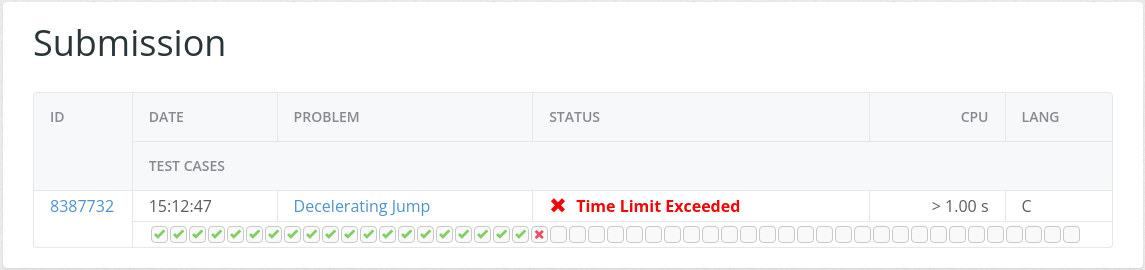
\includegraphics[scale = 0.25]{fig/tle1.png}
	}
}

\env{frame}
{
	\env{itemize}
	{
		\item<1-> Útfærum nú lausnina neðansækið í von um að geta bætt hana síðan.
		\item<2-> Munum að
		\[
			f(i, j) = 
			\left \{
			\env{array}
			{
				{l l}
				a_n, & \text{ef $i = n$},\\
				\max\limits_{1 \leq k \leq \min(j, n - i)} f(i + k, k) + a_i, & \text{annars}.
			}
			\right .
		\]
		\item<3-> Nú er $f(i, j)$ bara háð styttri stökkum eða jafn löngum stökkum sem byrja aftar.
		\item<4-> Svo við getum reiknað út $f(i, j)$ í vaxandi stökk röð, og minnkandi upphafsstöðum.
		\item<5-> Með öðrum orðum látum við $j$ vaxa, og $i$ minnka.
	}
}

\env{frame}
{
	\code{code/minnkandistokk-bu-slow.c}
}

\env{frame}
{
	\env{itemize}
	{
		\item<1-> Nú er þetta forrit lítið annað en þreföld \texttt{for}-lykkja, hver af lengd $\mathcal{O}(\,n\,)$.
		\item<2-> Svo tímaflækjan er $\mathcal{O}($\onslide<3->{$n^3$}$)$.
		\item<4-> Þetta ætti því einnig að vera of hægt.
		\item<5->[] 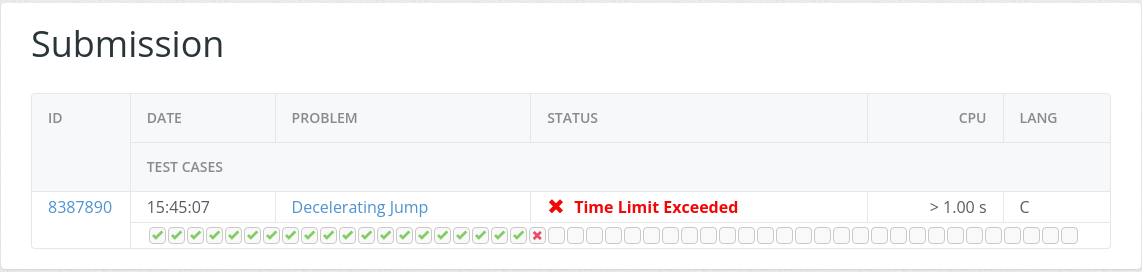
\includegraphics[scale = 0.25]{fig/tle2.png}
		\item<6-> Tökum þó eftir einu.
	}
}

\env{frame}
{
	\env{itemize}
	{
		\item<1-> Þegar við reiknum fallgildið $f(i, j)$ þá tökum við stærsta gildið á skálínunni $f(i + 1, 1), f(i + 2, 2), \dots, f(i + k, k)$.
		\item<2-> Eftir að hafa reiknað fallgildin fyrir tiltekna stökklengd hefur eitt stak bæst við hverja skálínu.
		\item<3-> Það er lítið mál að halda utan um stærsta stakið á hverri skálínu með því að uppfæra eftir að nýtt fallgildi er reiknað.
		\item<4-> Þá getum við líka reiknað hvert fallgildi í föstum tíma.
	}
}

\env{frame}
{
	\code{code/minnkandistokk.c}
}

\env{frame}
{
	\env{itemize}
	{
		\item<1-> Nú er þetta forrit lítið annað en tvöföld \texttt{for}-lykkja, hvor af lengd $\mathcal{O}(\,n\,)$.
		\item<2-> Svo tímaflækjan er $\mathcal{O}($\onslide<3->{$n^2$}$)$.
		\item<4-> Þetta ætti sleppa, því $(3 \cdot 10^3)^2 = 9 \cdot 10^6 < 10^8$.
		\item<5->[] 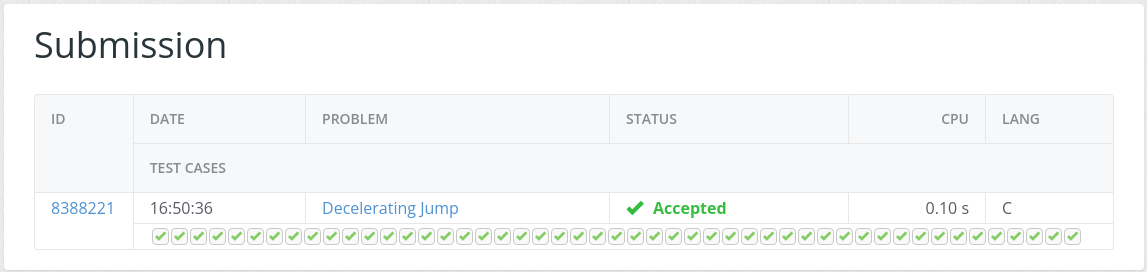
\includegraphics[scale = 0.25]{fig/ac.png}
	}
}

\env{frame}
{
}

\end{document}
